% Created by tikzDevice version 0.12.3 on 2019-09-30 10:38:03
% !TEX encoding = UTF-8 Unicode
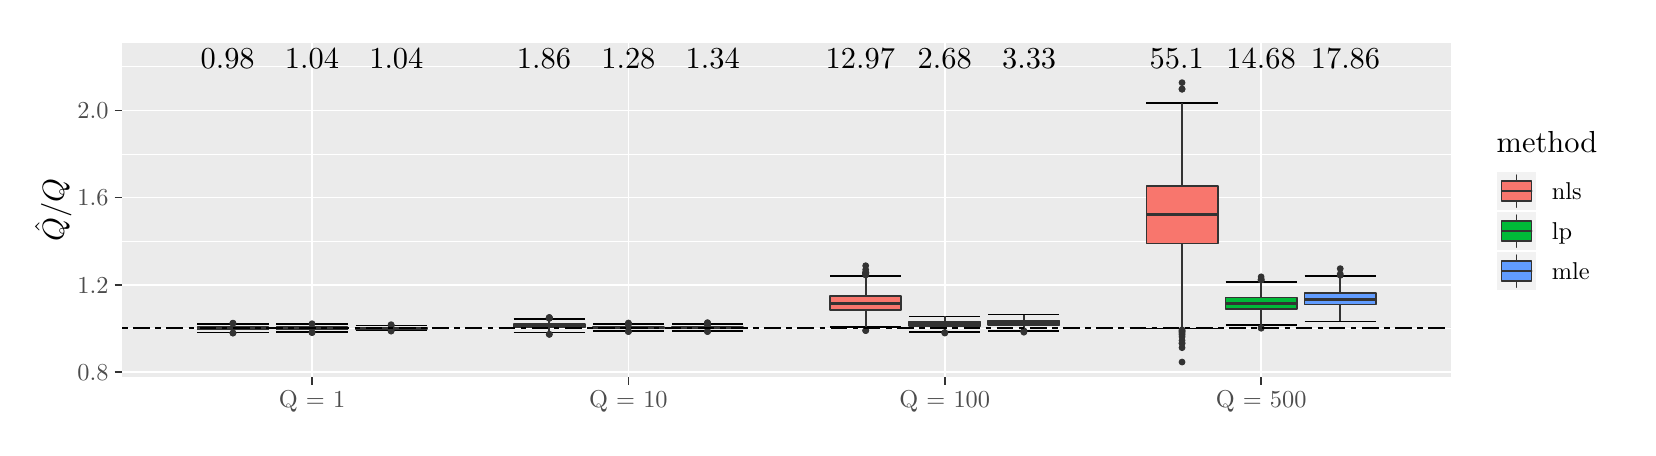
\begin{tikzpicture}[x=1pt,y=1pt]
\definecolor{fillColor}{RGB}{255,255,255}
\path[use as bounding box,fill=fillColor,fill opacity=0.00] (0,0) rectangle (578.16,144.54);
\begin{scope}
\path[clip] (  0.00,  0.00) rectangle (578.16,144.54);
\definecolor{drawColor}{RGB}{255,255,255}
\definecolor{fillColor}{RGB}{255,255,255}

\path[draw=drawColor,line width= 0.6pt,line join=round,line cap=round,fill=fillColor] (  0.00,  0.00) rectangle (578.16,144.54);
\end{scope}
\begin{scope}
\path[clip] ( 34.16, 18.22) rectangle (514.31,139.04);
\definecolor{fillColor}{gray}{0.92}

\path[fill=fillColor] ( 34.16, 18.22) rectangle (514.31,139.04);
\definecolor{drawColor}{RGB}{255,255,255}

\path[draw=drawColor,line width= 0.3pt,line join=round] ( 34.16, 35.91) --
	(514.31, 35.91);

\path[draw=drawColor,line width= 0.3pt,line join=round] ( 34.16, 67.40) --
	(514.31, 67.40);

\path[draw=drawColor,line width= 0.3pt,line join=round] ( 34.16, 98.89) --
	(514.31, 98.89);

\path[draw=drawColor,line width= 0.3pt,line join=round] ( 34.16,130.39) --
	(514.31,130.39);

\path[draw=drawColor,line width= 0.6pt,line join=round] ( 34.16, 20.16) --
	(514.31, 20.16);

\path[draw=drawColor,line width= 0.6pt,line join=round] ( 34.16, 51.65) --
	(514.31, 51.65);

\path[draw=drawColor,line width= 0.6pt,line join=round] ( 34.16, 83.15) --
	(514.31, 83.15);

\path[draw=drawColor,line width= 0.6pt,line join=round] ( 34.16,114.64) --
	(514.31,114.64);

\path[draw=drawColor,line width= 0.6pt,line join=round] (102.75, 18.22) --
	(102.75,139.04);

\path[draw=drawColor,line width= 0.6pt,line join=round] (217.07, 18.22) --
	(217.07,139.04);

\path[draw=drawColor,line width= 0.6pt,line join=round] (331.39, 18.22) --
	(331.39,139.04);

\path[draw=drawColor,line width= 0.6pt,line join=round] (445.71, 18.22) --
	(445.71,139.04);
\definecolor{drawColor}{RGB}{0,0,0}

\path[draw=drawColor,line width= 0.6pt,line join=round] ( 61.31, 37.57) --
	( 87.03, 37.57);

\path[draw=drawColor,line width= 0.6pt,line join=round] ( 74.17, 37.57) --
	( 74.17, 34.35);

\path[draw=drawColor,line width= 0.6pt,line join=round] ( 61.31, 34.35) --
	( 87.03, 34.35);

\path[draw=drawColor,line width= 0.6pt,line join=round] ( 89.89, 37.43) --
	(115.61, 37.43);

\path[draw=drawColor,line width= 0.6pt,line join=round] (102.75, 37.43) --
	(102.75, 34.47);

\path[draw=drawColor,line width= 0.6pt,line join=round] ( 89.89, 34.47) --
	(115.61, 34.47);

\path[draw=drawColor,line width= 0.6pt,line join=round] (118.47, 36.86) --
	(144.19, 36.86);

\path[draw=drawColor,line width= 0.6pt,line join=round] (131.33, 36.86) --
	(131.33, 35.09);

\path[draw=drawColor,line width= 0.6pt,line join=round] (118.47, 35.09) --
	(144.19, 35.09);

\path[draw=drawColor,line width= 0.6pt,line join=round] (175.63, 39.30) --
	(201.35, 39.30);

\path[draw=drawColor,line width= 0.6pt,line join=round] (188.49, 39.30) --
	(188.49, 34.37);

\path[draw=drawColor,line width= 0.6pt,line join=round] (175.63, 34.37) --
	(201.35, 34.37);

\path[draw=drawColor,line width= 0.6pt,line join=round] (204.21, 37.43) --
	(229.93, 37.43);

\path[draw=drawColor,line width= 0.6pt,line join=round] (217.07, 37.43) --
	(217.07, 34.92);

\path[draw=drawColor,line width= 0.6pt,line join=round] (204.21, 34.92) --
	(229.93, 34.92);

\path[draw=drawColor,line width= 0.6pt,line join=round] (232.79, 37.42) --
	(258.51, 37.42);

\path[draw=drawColor,line width= 0.6pt,line join=round] (245.65, 37.42) --
	(245.65, 34.96);

\path[draw=drawColor,line width= 0.6pt,line join=round] (232.79, 34.96) --
	(258.51, 34.96);

\path[draw=drawColor,line width= 0.6pt,line join=round] (289.95, 54.74) --
	(315.67, 54.74);

\path[draw=drawColor,line width= 0.6pt,line join=round] (302.81, 54.74) --
	(302.81, 36.48);

\path[draw=drawColor,line width= 0.6pt,line join=round] (289.95, 36.48) --
	(315.67, 36.48);

\path[draw=drawColor,line width= 0.6pt,line join=round] (318.53, 40.18) --
	(344.25, 40.18);

\path[draw=drawColor,line width= 0.6pt,line join=round] (331.39, 40.18) --
	(331.39, 34.53);

\path[draw=drawColor,line width= 0.6pt,line join=round] (318.53, 34.53) --
	(344.25, 34.53);

\path[draw=drawColor,line width= 0.6pt,line join=round] (347.11, 40.84) --
	(372.83, 40.84);

\path[draw=drawColor,line width= 0.6pt,line join=round] (359.97, 40.84) --
	(359.97, 35.04);

\path[draw=drawColor,line width= 0.6pt,line join=round] (347.11, 35.04) --
	(372.83, 35.04);

\path[draw=drawColor,line width= 0.6pt,line join=round] (404.27,117.30) --
	(430.00,117.30);

\path[draw=drawColor,line width= 0.6pt,line join=round] (417.13,117.30) --
	(417.13, 35.85);

\path[draw=drawColor,line width= 0.6pt,line join=round] (404.27, 35.85) --
	(430.00, 35.85);

\path[draw=drawColor,line width= 0.6pt,line join=round] (432.85, 52.65) --
	(458.58, 52.65);

\path[draw=drawColor,line width= 0.6pt,line join=round] (445.71, 52.65) --
	(445.71, 37.17);

\path[draw=drawColor,line width= 0.6pt,line join=round] (432.85, 37.17) --
	(458.58, 37.17);

\path[draw=drawColor,line width= 0.6pt,line join=round] (461.43, 54.77) --
	(487.16, 54.77);

\path[draw=drawColor,line width= 0.6pt,line join=round] (474.29, 54.77) --
	(474.29, 38.41);

\path[draw=drawColor,line width= 0.6pt,line join=round] (461.43, 38.41) --
	(487.16, 38.41);
\definecolor{drawColor}{gray}{0.20}
\definecolor{fillColor}{gray}{0.20}

\path[draw=drawColor,line width= 0.4pt,line join=round,line cap=round,fill=fillColor] ( 74.17, 37.77) circle (  1.02);

\path[draw=drawColor,line width= 0.4pt,line join=round,line cap=round,fill=fillColor] ( 74.17, 34.19) circle (  1.02);

\path[draw=drawColor,line width= 0.4pt,line join=round,line cap=round,fill=fillColor] ( 74.17, 34.19) circle (  1.02);

\path[draw=drawColor,line width= 0.4pt,line join=round,line cap=round,fill=fillColor] ( 74.17, 37.71) circle (  1.02);

\path[draw=drawColor,line width= 0.6pt,line join=round] ( 74.17, 36.32) -- ( 74.17, 37.57);

\path[draw=drawColor,line width= 0.6pt,line join=round] ( 74.17, 35.48) -- ( 74.17, 34.35);
\definecolor{fillColor}{RGB}{248,118,109}

\path[draw=drawColor,line width= 0.6pt,line join=round,line cap=round,fill=fillColor] ( 61.31, 36.32) --
	( 61.31, 35.48) --
	( 87.03, 35.48) --
	( 87.03, 36.32) --
	( 61.31, 36.32) --
	cycle;

\path[draw=drawColor,line width= 1.1pt,line join=round] ( 61.31, 35.88) -- ( 87.03, 35.88);
\definecolor{fillColor}{gray}{0.20}

\path[draw=drawColor,line width= 0.4pt,line join=round,line cap=round,fill=fillColor] (102.75, 34.39) circle (  1.02);

\path[draw=drawColor,line width= 0.4pt,line join=round,line cap=round,fill=fillColor] (102.75, 37.56) circle (  1.02);

\path[draw=drawColor,line width= 0.4pt,line join=round,line cap=round,fill=fillColor] (102.75, 34.37) circle (  1.02);

\path[draw=drawColor,line width= 0.6pt,line join=round] (102.75, 36.33) -- (102.75, 37.43);

\path[draw=drawColor,line width= 0.6pt,line join=round] (102.75, 35.58) -- (102.75, 34.47);
\definecolor{fillColor}{RGB}{0,186,56}

\path[draw=drawColor,line width= 0.6pt,line join=round,line cap=round,fill=fillColor] ( 89.89, 36.33) --
	( 89.89, 35.58) --
	(115.61, 35.58) --
	(115.61, 36.33) --
	( 89.89, 36.33) --
	cycle;

\path[draw=drawColor,line width= 1.1pt,line join=round] ( 89.89, 35.95) -- (115.61, 35.95);
\definecolor{fillColor}{gray}{0.20}

\path[draw=drawColor,line width= 0.4pt,line join=round,line cap=round,fill=fillColor] (131.33, 34.99) circle (  1.02);

\path[draw=drawColor,line width= 0.4pt,line join=round,line cap=round,fill=fillColor] (131.33, 36.91) circle (  1.02);

\path[draw=drawColor,line width= 0.4pt,line join=round,line cap=round,fill=fillColor] (131.33, 36.95) circle (  1.02);

\path[draw=drawColor,line width= 0.4pt,line join=round,line cap=round,fill=fillColor] (131.33, 37.22) circle (  1.02);

\path[draw=drawColor,line width= 0.4pt,line join=round,line cap=round,fill=fillColor] (131.33, 36.92) circle (  1.02);

\path[draw=drawColor,line width= 0.4pt,line join=round,line cap=round,fill=fillColor] (131.33, 34.90) circle (  1.02);

\path[draw=drawColor,line width= 0.6pt,line join=round] (131.33, 36.19) -- (131.33, 36.86);

\path[draw=drawColor,line width= 0.6pt,line join=round] (131.33, 35.74) -- (131.33, 35.09);
\definecolor{fillColor}{RGB}{97,156,255}

\path[draw=drawColor,line width= 0.6pt,line join=round,line cap=round,fill=fillColor] (118.47, 36.19) --
	(118.47, 35.74) --
	(144.19, 35.74) --
	(144.19, 36.19) --
	(118.47, 36.19) --
	cycle;

\path[draw=drawColor,line width= 1.1pt,line join=round] (118.47, 35.94) -- (144.19, 35.94);
\definecolor{fillColor}{gray}{0.20}

\path[draw=drawColor,line width= 0.4pt,line join=round,line cap=round,fill=fillColor] (188.49, 39.56) circle (  1.02);

\path[draw=drawColor,line width= 0.4pt,line join=round,line cap=round,fill=fillColor] (188.49, 33.73) circle (  1.02);

\path[draw=drawColor,line width= 0.4pt,line join=round,line cap=round,fill=fillColor] (188.49, 39.59) circle (  1.02);

\path[draw=drawColor,line width= 0.4pt,line join=round,line cap=round,fill=fillColor] (188.49, 39.77) circle (  1.02);

\path[draw=drawColor,line width= 0.4pt,line join=round,line cap=round,fill=fillColor] (188.49, 39.53) circle (  1.02);

\path[draw=drawColor,line width= 0.4pt,line join=round,line cap=round,fill=fillColor] (188.49, 33.72) circle (  1.02);

\path[draw=drawColor,line width= 0.4pt,line join=round,line cap=round,fill=fillColor] (188.49, 39.81) circle (  1.02);

\path[draw=drawColor,line width= 0.4pt,line join=round,line cap=round,fill=fillColor] (188.49, 39.70) circle (  1.02);

\path[draw=drawColor,line width= 0.6pt,line join=round] (188.49, 37.45) -- (188.49, 39.30);

\path[draw=drawColor,line width= 0.6pt,line join=round] (188.49, 36.18) -- (188.49, 34.37);
\definecolor{fillColor}{RGB}{248,118,109}

\path[draw=drawColor,line width= 0.6pt,line join=round,line cap=round,fill=fillColor] (175.63, 37.45) --
	(175.63, 36.18) --
	(201.35, 36.18) --
	(201.35, 37.45) --
	(175.63, 37.45) --
	cycle;

\path[draw=drawColor,line width= 1.1pt,line join=round] (175.63, 36.82) -- (201.35, 36.82);
\definecolor{fillColor}{gray}{0.20}

\path[draw=drawColor,line width= 0.4pt,line join=round,line cap=round,fill=fillColor] (217.07, 34.76) circle (  1.02);

\path[draw=drawColor,line width= 0.4pt,line join=round,line cap=round,fill=fillColor] (217.07, 37.43) circle (  1.02);

\path[draw=drawColor,line width= 0.4pt,line join=round,line cap=round,fill=fillColor] (217.07, 34.78) circle (  1.02);

\path[draw=drawColor,line width= 0.4pt,line join=round,line cap=round,fill=fillColor] (217.07, 37.56) circle (  1.02);

\path[draw=drawColor,line width= 0.4pt,line join=round,line cap=round,fill=fillColor] (217.07, 34.77) circle (  1.02);

\path[draw=drawColor,line width= 0.4pt,line join=round,line cap=round,fill=fillColor] (217.07, 37.47) circle (  1.02);

\path[draw=drawColor,line width= 0.4pt,line join=round,line cap=round,fill=fillColor] (217.07, 37.82) circle (  1.02);

\path[draw=drawColor,line width= 0.4pt,line join=round,line cap=round,fill=fillColor] (217.07, 37.52) circle (  1.02);

\path[draw=drawColor,line width= 0.6pt,line join=round] (217.07, 36.44) -- (217.07, 37.43);

\path[draw=drawColor,line width= 0.6pt,line join=round] (217.07, 35.78) -- (217.07, 34.92);
\definecolor{fillColor}{RGB}{0,186,56}

\path[draw=drawColor,line width= 0.6pt,line join=round,line cap=round,fill=fillColor] (204.21, 36.44) --
	(204.21, 35.78) --
	(229.93, 35.78) --
	(229.93, 36.44) --
	(204.21, 36.44) --
	cycle;

\path[draw=drawColor,line width= 1.1pt,line join=round] (204.21, 36.12) -- (229.93, 36.12);
\definecolor{fillColor}{gray}{0.20}

\path[draw=drawColor,line width= 0.4pt,line join=round,line cap=round,fill=fillColor] (245.65, 34.73) circle (  1.02);

\path[draw=drawColor,line width= 0.4pt,line join=round,line cap=round,fill=fillColor] (245.65, 37.44) circle (  1.02);

\path[draw=drawColor,line width= 0.4pt,line join=round,line cap=round,fill=fillColor] (245.65, 34.80) circle (  1.02);

\path[draw=drawColor,line width= 0.4pt,line join=round,line cap=round,fill=fillColor] (245.65, 37.79) circle (  1.02);

\path[draw=drawColor,line width= 0.4pt,line join=round,line cap=round,fill=fillColor] (245.65, 34.83) circle (  1.02);

\path[draw=drawColor,line width= 0.4pt,line join=round,line cap=round,fill=fillColor] (245.65, 37.51) circle (  1.02);

\path[draw=drawColor,line width= 0.4pt,line join=round,line cap=round,fill=fillColor] (245.65, 37.95) circle (  1.02);

\path[draw=drawColor,line width= 0.4pt,line join=round,line cap=round,fill=fillColor] (245.65, 37.49) circle (  1.02);

\path[draw=drawColor,line width= 0.4pt,line join=round,line cap=round,fill=fillColor] (245.65, 37.45) circle (  1.02);

\path[draw=drawColor,line width= 0.4pt,line join=round,line cap=round,fill=fillColor] (245.65, 37.43) circle (  1.02);

\path[draw=drawColor,line width= 0.4pt,line join=round,line cap=round,fill=fillColor] (245.65, 37.76) circle (  1.02);

\path[draw=drawColor,line width= 0.4pt,line join=round,line cap=round,fill=fillColor] (245.65, 37.59) circle (  1.02);

\path[draw=drawColor,line width= 0.6pt,line join=round] (245.65, 36.48) -- (245.65, 37.42);

\path[draw=drawColor,line width= 0.6pt,line join=round] (245.65, 35.86) -- (245.65, 34.96);
\definecolor{fillColor}{RGB}{97,156,255}

\path[draw=drawColor,line width= 0.6pt,line join=round,line cap=round,fill=fillColor] (232.79, 36.48) --
	(232.79, 35.86) --
	(258.51, 35.86) --
	(258.51, 36.48) --
	(232.79, 36.48) --
	cycle;

\path[draw=drawColor,line width= 1.1pt,line join=round] (232.79, 36.17) -- (258.51, 36.17);
\definecolor{fillColor}{gray}{0.20}

\path[draw=drawColor,line width= 0.4pt,line join=round,line cap=round,fill=fillColor] (302.81, 56.00) circle (  1.02);

\path[draw=drawColor,line width= 0.4pt,line join=round,line cap=round,fill=fillColor] (302.81, 35.13) circle (  1.02);

\path[draw=drawColor,line width= 0.4pt,line join=round,line cap=round,fill=fillColor] (302.81, 57.11) circle (  1.02);

\path[draw=drawColor,line width= 0.4pt,line join=round,line cap=round,fill=fillColor] (302.81, 55.72) circle (  1.02);

\path[draw=drawColor,line width= 0.4pt,line join=round,line cap=round,fill=fillColor] (302.81, 55.51) circle (  1.02);

\path[draw=drawColor,line width= 0.4pt,line join=round,line cap=round,fill=fillColor] (302.81, 58.53) circle (  1.02);

\path[draw=drawColor,line width= 0.4pt,line join=round,line cap=round,fill=fillColor] (302.81, 56.07) circle (  1.02);

\path[draw=drawColor,line width= 0.4pt,line join=round,line cap=round,fill=fillColor] (302.81, 55.81) circle (  1.02);

\path[draw=drawColor,line width= 0.4pt,line join=round,line cap=round,fill=fillColor] (302.81, 56.07) circle (  1.02);

\path[draw=drawColor,line width= 0.4pt,line join=round,line cap=round,fill=fillColor] (302.81, 55.16) circle (  1.02);

\path[draw=drawColor,line width= 0.4pt,line join=round,line cap=round,fill=fillColor] (302.81, 35.07) circle (  1.02);

\path[draw=drawColor,line width= 0.6pt,line join=round] (302.81, 47.51) -- (302.81, 54.74);

\path[draw=drawColor,line width= 0.6pt,line join=round] (302.81, 42.56) -- (302.81, 36.48);
\definecolor{fillColor}{RGB}{248,118,109}

\path[draw=drawColor,line width= 0.6pt,line join=round,line cap=round,fill=fillColor] (289.95, 47.51) --
	(289.95, 42.56) --
	(315.67, 42.56) --
	(315.67, 47.51) --
	(289.95, 47.51) --
	cycle;

\path[draw=drawColor,line width= 1.1pt,line join=round] (289.95, 44.96) -- (315.67, 44.96);
\definecolor{fillColor}{gray}{0.20}

\path[draw=drawColor,line width= 0.4pt,line join=round,line cap=round,fill=fillColor] (331.39, 34.19) circle (  1.02);

\path[draw=drawColor,line width= 0.4pt,line join=round,line cap=round,fill=fillColor] (331.39, 34.39) circle (  1.02);

\path[draw=drawColor,line width= 0.6pt,line join=round] (331.39, 38.33) -- (331.39, 40.18);

\path[draw=drawColor,line width= 0.6pt,line join=round] (331.39, 36.78) -- (331.39, 34.53);
\definecolor{fillColor}{RGB}{0,186,56}

\path[draw=drawColor,line width= 0.6pt,line join=round,line cap=round,fill=fillColor] (318.53, 38.33) --
	(318.53, 36.78) --
	(344.25, 36.78) --
	(344.25, 38.33) --
	(318.53, 38.33) --
	cycle;

\path[draw=drawColor,line width= 1.1pt,line join=round] (318.53, 37.59) -- (344.25, 37.59);
\definecolor{fillColor}{gray}{0.20}

\path[draw=drawColor,line width= 0.4pt,line join=round,line cap=round,fill=fillColor] (359.97, 34.50) circle (  1.02);

\path[draw=drawColor,line width= 0.4pt,line join=round,line cap=round,fill=fillColor] (359.97, 34.81) circle (  1.02);

\path[draw=drawColor,line width= 0.4pt,line join=round,line cap=round,fill=fillColor] (359.97, 34.86) circle (  1.02);

\path[draw=drawColor,line width= 0.4pt,line join=round,line cap=round,fill=fillColor] (359.97, 34.82) circle (  1.02);

\path[draw=drawColor,line width= 0.4pt,line join=round,line cap=round,fill=fillColor] (359.97, 34.97) circle (  1.02);

\path[draw=drawColor,line width= 0.6pt,line join=round] (359.97, 38.68) -- (359.97, 40.84);

\path[draw=drawColor,line width= 0.6pt,line join=round] (359.97, 37.20) -- (359.97, 35.04);
\definecolor{fillColor}{RGB}{97,156,255}

\path[draw=drawColor,line width= 0.6pt,line join=round,line cap=round,fill=fillColor] (347.11, 38.68) --
	(347.11, 37.20) --
	(372.83, 37.20) --
	(372.83, 38.68) --
	(347.11, 38.68) --
	cycle;

\path[draw=drawColor,line width= 1.1pt,line join=round] (347.11, 37.96) -- (372.83, 37.96);
\definecolor{fillColor}{gray}{0.20}

\path[draw=drawColor,line width= 0.4pt,line join=round,line cap=round,fill=fillColor] (417.13, 32.84) circle (  1.02);

\path[draw=drawColor,line width= 0.4pt,line join=round,line cap=round,fill=fillColor] (417.13, 23.71) circle (  1.02);

\path[draw=drawColor,line width= 0.4pt,line join=round,line cap=round,fill=fillColor] (417.13, 35.04) circle (  1.02);

\path[draw=drawColor,line width= 0.4pt,line join=round,line cap=round,fill=fillColor] (417.13,122.28) circle (  1.02);

\path[draw=drawColor,line width= 0.4pt,line join=round,line cap=round,fill=fillColor] (417.13, 30.55) circle (  1.02);

\path[draw=drawColor,line width= 0.4pt,line join=round,line cap=round,fill=fillColor] (417.13,122.40) circle (  1.02);

\path[draw=drawColor,line width= 0.4pt,line join=round,line cap=round,fill=fillColor] (417.13, 35.35) circle (  1.02);

\path[draw=drawColor,line width= 0.4pt,line join=round,line cap=round,fill=fillColor] (417.13, 31.52) circle (  1.02);

\path[draw=drawColor,line width= 0.4pt,line join=round,line cap=round,fill=fillColor] (417.13, 33.92) circle (  1.02);

\path[draw=drawColor,line width= 0.4pt,line join=round,line cap=round,fill=fillColor] (417.13, 33.54) circle (  1.02);

\path[draw=drawColor,line width= 0.4pt,line join=round,line cap=round,fill=fillColor] (417.13, 34.44) circle (  1.02);

\path[draw=drawColor,line width= 0.4pt,line join=round,line cap=round,fill=fillColor] (417.13, 30.44) circle (  1.02);

\path[draw=drawColor,line width= 0.4pt,line join=round,line cap=round,fill=fillColor] (417.13,124.67) circle (  1.02);

\path[draw=drawColor,line width= 0.4pt,line join=round,line cap=round,fill=fillColor] (417.13, 34.79) circle (  1.02);

\path[draw=drawColor,line width= 0.4pt,line join=round,line cap=round,fill=fillColor] (417.13, 28.90) circle (  1.02);

\path[draw=drawColor,line width= 0.6pt,line join=round] (417.13, 87.35) -- (417.13,117.30);

\path[draw=drawColor,line width= 0.6pt,line join=round] (417.13, 66.60) -- (417.13, 35.85);
\definecolor{fillColor}{RGB}{248,118,109}

\path[draw=drawColor,line width= 0.6pt,line join=round,line cap=round,fill=fillColor] (404.27, 87.35) --
	(404.27, 66.60) --
	(430.00, 66.60) --
	(430.00, 87.35) --
	(404.27, 87.35) --
	cycle;

\path[draw=drawColor,line width= 1.1pt,line join=round] (404.27, 76.94) -- (430.00, 76.94);
\definecolor{fillColor}{gray}{0.20}

\path[draw=drawColor,line width= 0.4pt,line join=round,line cap=round,fill=fillColor] (445.71, 35.93) circle (  1.02);

\path[draw=drawColor,line width= 0.4pt,line join=round,line cap=round,fill=fillColor] (445.71, 36.14) circle (  1.02);

\path[draw=drawColor,line width= 0.4pt,line join=round,line cap=round,fill=fillColor] (445.71, 53.35) circle (  1.02);

\path[draw=drawColor,line width= 0.4pt,line join=round,line cap=round,fill=fillColor] (445.71, 53.66) circle (  1.02);

\path[draw=drawColor,line width= 0.4pt,line join=round,line cap=round,fill=fillColor] (445.71, 53.35) circle (  1.02);

\path[draw=drawColor,line width= 0.4pt,line join=round,line cap=round,fill=fillColor] (445.71, 54.51) circle (  1.02);

\path[draw=drawColor,line width= 0.4pt,line join=round,line cap=round,fill=fillColor] (445.71, 53.45) circle (  1.02);

\path[draw=drawColor,line width= 0.6pt,line join=round] (445.71, 46.99) -- (445.71, 52.65);

\path[draw=drawColor,line width= 0.6pt,line join=round] (445.71, 42.81) -- (445.71, 37.17);
\definecolor{fillColor}{RGB}{0,186,56}

\path[draw=drawColor,line width= 0.6pt,line join=round,line cap=round,fill=fillColor] (432.85, 46.99) --
	(432.85, 42.81) --
	(458.58, 42.81) --
	(458.58, 46.99) --
	(432.85, 46.99) --
	cycle;

\path[draw=drawColor,line width= 1.1pt,line join=round] (432.85, 44.96) -- (458.58, 44.96);
\definecolor{fillColor}{gray}{0.20}

\path[draw=drawColor,line width= 0.4pt,line join=round,line cap=round,fill=fillColor] (474.29, 57.47) circle (  1.02);

\path[draw=drawColor,line width= 0.4pt,line join=round,line cap=round,fill=fillColor] (474.29, 55.06) circle (  1.02);

\path[draw=drawColor,line width= 0.4pt,line join=round,line cap=round,fill=fillColor] (474.29, 55.56) circle (  1.02);

\path[draw=drawColor,line width= 0.6pt,line join=round] (474.29, 48.60) -- (474.29, 54.77);

\path[draw=drawColor,line width= 0.6pt,line join=round] (474.29, 44.46) -- (474.29, 38.41);
\definecolor{fillColor}{RGB}{97,156,255}

\path[draw=drawColor,line width= 0.6pt,line join=round,line cap=round,fill=fillColor] (461.43, 48.60) --
	(461.43, 44.46) --
	(487.16, 44.46) --
	(487.16, 48.60) --
	(461.43, 48.60) --
	cycle;

\path[draw=drawColor,line width= 1.1pt,line join=round] (461.43, 46.40) -- (487.16, 46.40);
\definecolor{drawColor}{RGB}{0,0,0}

\path[draw=drawColor,line width= 0.6pt,dash pattern=on 2pt off 2pt on 6pt off 2pt ,line join=round] ( 34.16, 35.91) -- (514.31, 35.91);

\node[text=drawColor,anchor=base,inner sep=0pt, outer sep=0pt, scale=  1.10] at (133.23,129.75) {1.04};

\node[text=drawColor,anchor=base,inner sep=0pt, outer sep=0pt, scale=  1.10] at (102.75,129.75) {1.04};

\node[text=drawColor,anchor=base,inner sep=0pt, outer sep=0pt, scale=  1.10] at ( 72.26,129.75) {0.98};

\node[text=drawColor,anchor=base,inner sep=0pt, outer sep=0pt, scale=  1.10] at (247.56,129.75) {1.34};

\node[text=drawColor,anchor=base,inner sep=0pt, outer sep=0pt, scale=  1.10] at (217.07,129.75) {1.28};

\node[text=drawColor,anchor=base,inner sep=0pt, outer sep=0pt, scale=  1.10] at (186.59,129.75) {1.86};

\node[text=drawColor,anchor=base,inner sep=0pt, outer sep=0pt, scale=  1.10] at (361.88,129.75) {3.33};

\node[text=drawColor,anchor=base,inner sep=0pt, outer sep=0pt, scale=  1.10] at (331.39,129.75) {2.68};

\node[text=drawColor,anchor=base,inner sep=0pt, outer sep=0pt, scale=  1.10] at (300.91,129.75) {12.97};

\node[text=drawColor,anchor=base,inner sep=0pt, outer sep=0pt, scale=  1.10] at (476.20,129.75) {17.86};

\node[text=drawColor,anchor=base,inner sep=0pt, outer sep=0pt, scale=  1.10] at (445.71,129.75) {14.68};

\node[text=drawColor,anchor=base,inner sep=0pt, outer sep=0pt, scale=  1.10] at (415.23,129.75) {55.1};
\end{scope}
\begin{scope}
\path[clip] (  0.00,  0.00) rectangle (578.16,144.54);
\definecolor{drawColor}{gray}{0.30}

\node[text=drawColor,anchor=base east,inner sep=0pt, outer sep=0pt, scale=  0.88] at ( 29.21, 17.13) {0.8};

\node[text=drawColor,anchor=base east,inner sep=0pt, outer sep=0pt, scale=  0.88] at ( 29.21, 48.62) {1.2};

\node[text=drawColor,anchor=base east,inner sep=0pt, outer sep=0pt, scale=  0.88] at ( 29.21, 80.12) {1.6};

\node[text=drawColor,anchor=base east,inner sep=0pt, outer sep=0pt, scale=  0.88] at ( 29.21,111.61) {2.0};
\end{scope}
\begin{scope}
\path[clip] (  0.00,  0.00) rectangle (578.16,144.54);
\definecolor{drawColor}{gray}{0.20}

\path[draw=drawColor,line width= 0.6pt,line join=round] ( 31.41, 20.16) --
	( 34.16, 20.16);

\path[draw=drawColor,line width= 0.6pt,line join=round] ( 31.41, 51.65) --
	( 34.16, 51.65);

\path[draw=drawColor,line width= 0.6pt,line join=round] ( 31.41, 83.15) --
	( 34.16, 83.15);

\path[draw=drawColor,line width= 0.6pt,line join=round] ( 31.41,114.64) --
	( 34.16,114.64);
\end{scope}
\begin{scope}
\path[clip] (  0.00,  0.00) rectangle (578.16,144.54);
\definecolor{drawColor}{gray}{0.20}

\path[draw=drawColor,line width= 0.6pt,line join=round] (102.75, 15.47) --
	(102.75, 18.22);

\path[draw=drawColor,line width= 0.6pt,line join=round] (217.07, 15.47) --
	(217.07, 18.22);

\path[draw=drawColor,line width= 0.6pt,line join=round] (331.39, 15.47) --
	(331.39, 18.22);

\path[draw=drawColor,line width= 0.6pt,line join=round] (445.71, 15.47) --
	(445.71, 18.22);
\end{scope}
\begin{scope}
\path[clip] (  0.00,  0.00) rectangle (578.16,144.54);
\definecolor{drawColor}{gray}{0.30}

\node[text=drawColor,anchor=base,inner sep=0pt, outer sep=0pt, scale=  0.88] at (102.75,  7.21) {Q = 1};

\node[text=drawColor,anchor=base,inner sep=0pt, outer sep=0pt, scale=  0.88] at (217.07,  7.21) {Q = 10};

\node[text=drawColor,anchor=base,inner sep=0pt, outer sep=0pt, scale=  0.88] at (331.39,  7.21) {Q = 100};

\node[text=drawColor,anchor=base,inner sep=0pt, outer sep=0pt, scale=  0.88] at (445.71,  7.21) {Q = 500};
\end{scope}
\begin{scope}
\path[clip] (  0.00,  0.00) rectangle (578.16,144.54);
\definecolor{drawColor}{RGB}{0,0,0}

\node[text=drawColor,rotate= 90.00,anchor=base,inner sep=0pt, outer sep=0pt, scale=  1.10] at ( 13.08, 78.63) {$\hat{Q}/Q$};
\end{scope}
\begin{scope}
\path[clip] (  0.00,  0.00) rectangle (578.16,144.54);
\definecolor{fillColor}{RGB}{255,255,255}

\path[fill=fillColor] (525.31, 43.84) rectangle (572.66,113.42);
\end{scope}
\begin{scope}
\path[clip] (  0.00,  0.00) rectangle (578.16,144.54);
\definecolor{drawColor}{RGB}{0,0,0}

\node[text=drawColor,anchor=base west,inner sep=0pt, outer sep=0pt, scale=  1.10] at (530.81, 99.27) {method};
\end{scope}
\begin{scope}
\path[clip] (  0.00,  0.00) rectangle (578.16,144.54);
\definecolor{drawColor}{RGB}{255,255,255}
\definecolor{fillColor}{gray}{0.95}

\path[draw=drawColor,line width= 0.6pt,line join=round,line cap=round,fill=fillColor] (530.81, 78.25) rectangle (545.26, 92.70);
\end{scope}
\begin{scope}
\path[clip] (  0.00,  0.00) rectangle (578.16,144.54);
\definecolor{drawColor}{gray}{0.20}

\path[draw=drawColor,line width= 0.6pt,line join=round,line cap=round] (538.03, 79.70) --
	(538.03, 81.86);

\path[draw=drawColor,line width= 0.6pt,line join=round,line cap=round] (538.03, 89.09) --
	(538.03, 91.26);
\definecolor{fillColor}{RGB}{248,118,109}

\path[draw=drawColor,line width= 0.6pt,line join=round,line cap=round,fill=fillColor] (532.61, 81.86) rectangle (543.45, 89.09);

\path[draw=drawColor,line width= 0.6pt,line join=round,line cap=round] (532.61, 85.48) --
	(543.45, 85.48);
\end{scope}
\begin{scope}
\path[clip] (  0.00,  0.00) rectangle (578.16,144.54);
\definecolor{drawColor}{RGB}{255,255,255}
\definecolor{fillColor}{gray}{0.95}

\path[draw=drawColor,line width= 0.6pt,line join=round,line cap=round,fill=fillColor] (530.81, 63.80) rectangle (545.26, 78.25);
\end{scope}
\begin{scope}
\path[clip] (  0.00,  0.00) rectangle (578.16,144.54);
\definecolor{drawColor}{gray}{0.20}

\path[draw=drawColor,line width= 0.6pt,line join=round,line cap=round] (538.03, 65.24) --
	(538.03, 67.41);

\path[draw=drawColor,line width= 0.6pt,line join=round,line cap=round] (538.03, 74.64) --
	(538.03, 76.81);
\definecolor{fillColor}{RGB}{0,186,56}

\path[draw=drawColor,line width= 0.6pt,line join=round,line cap=round,fill=fillColor] (532.61, 67.41) rectangle (543.45, 74.64);

\path[draw=drawColor,line width= 0.6pt,line join=round,line cap=round] (532.61, 71.02) --
	(543.45, 71.02);
\end{scope}
\begin{scope}
\path[clip] (  0.00,  0.00) rectangle (578.16,144.54);
\definecolor{drawColor}{RGB}{255,255,255}
\definecolor{fillColor}{gray}{0.95}

\path[draw=drawColor,line width= 0.6pt,line join=round,line cap=round,fill=fillColor] (530.81, 49.34) rectangle (545.26, 63.80);
\end{scope}
\begin{scope}
\path[clip] (  0.00,  0.00) rectangle (578.16,144.54);
\definecolor{drawColor}{gray}{0.20}

\path[draw=drawColor,line width= 0.6pt,line join=round,line cap=round] (538.03, 50.79) --
	(538.03, 52.96);

\path[draw=drawColor,line width= 0.6pt,line join=round,line cap=round] (538.03, 60.18) --
	(538.03, 62.35);
\definecolor{fillColor}{RGB}{97,156,255}

\path[draw=drawColor,line width= 0.6pt,line join=round,line cap=round,fill=fillColor] (532.61, 52.96) rectangle (543.45, 60.18);

\path[draw=drawColor,line width= 0.6pt,line join=round,line cap=round] (532.61, 56.57) --
	(543.45, 56.57);
\end{scope}
\begin{scope}
\path[clip] (  0.00,  0.00) rectangle (578.16,144.54);
\definecolor{drawColor}{RGB}{0,0,0}

\node[text=drawColor,anchor=base west,inner sep=0pt, outer sep=0pt, scale=  0.88] at (550.76, 82.45) {nls};
\end{scope}
\begin{scope}
\path[clip] (  0.00,  0.00) rectangle (578.16,144.54);
\definecolor{drawColor}{RGB}{0,0,0}

\node[text=drawColor,anchor=base west,inner sep=0pt, outer sep=0pt, scale=  0.88] at (550.76, 67.99) {lp};
\end{scope}
\begin{scope}
\path[clip] (  0.00,  0.00) rectangle (578.16,144.54);
\definecolor{drawColor}{RGB}{0,0,0}

\node[text=drawColor,anchor=base west,inner sep=0pt, outer sep=0pt, scale=  0.88] at (550.76, 53.54) {mle};
\end{scope}
\end{tikzpicture}
